
\documentclass[natbib,referee]{svjour3}

\smartqed  % flush right qed marks, e.g. at end of proof


% PACKAGES
% ------------------------------------------------------------------------------

\usepackage{simplemargins}
\usepackage{textcomp}
\usepackage{amsbsy}
\usepackage[dvipsnames]{xcolor}

\usepackage{graphicx}
\usepackage[pdftex,bookmarks=false]{hyperref}


% LINKS
% ------------------------------------------------------------------------------

\hypersetup{
    pdfpagelayout=OneColumn,
    colorlinks = true,
    urlcolor   = blue,
    citecolor  = blue,
    linkcolor  = blue
}
\urlstyle{same}


% ADDITIONAL COMMANDS
% ------------------------------------------------------------------------------

\newcommand{\myrevision}[1]{\textcolor{Green}{#1}}
\settopmargin{1.2in}
\setleftmargin{.9in}
\setrightmargin{1in}
\setbottommargin{.2in}


% JOURNAL NAME
% ------------------------------------------------------------------------------

\journalname{Pure and Applied Geophysics}


% MAIN DOCUMENT STARTS
% ==============================================================================

\begin{document}


% TITLE
% ------------------------------------------------------------------------------

\title{Analysis of the 2005--\myrevision{2016} earthquake sequence in northern Iran using the visibility graph method}
\titlerunning{Analysis of northern Iran seismicity using the visibility graph method}


% AUTHORS
% ------------------------------------------------------------------------------

\author{%
    Naeem Khoshnevis \and 
    Ricardo Taborda \newline
    Shima Azizzadeh-Roodpish \and 
    Luciano Telesca
}

% \authorrunning{N.~Khosh} % if too long for running head

\institute{
    N. Khoshnevis \and
    R. Taborda \and
    S. Azizzadeh-Roodpish 
    \at
        Center for Earthquake Research and Information\\
        The University of Memphis, Memphis, TN 38152, U.S.A.\\
        \email{nkhshnvs@memphis.edu}
    \and
    R. Taborda \and
    S. Azizzadeh-Roodpish 
        \at
        Department of Civil Engineering\\
        The University of Memphis, Memphis, TN 38152, U.S.A.
    \and
    L. Telesca
        \at
        Institute of Methodologies for Environmental Analysis\\
        National Research Council, Tito, Italy.
}

\date{Received: date / Accepted: date}

\maketitle

\begin{abstract}
    %
The seismicity of northern Iran between 2005 and 2015 is investigated by means of the visibility graph (VG) method. For purposes of this study, northern Iran is divided into three tectonic seismic regions: Azerbaijan, Alborz, and Kopeh Dagh. Using the declustered catalog, we studied the VG properties of the magnitude time series. The results show a relationship between the $k-M$ slope and the $b-value$ of the Gutenberg-Richter law. Topological properties (i.e.  $< T_c >$, $k-M$ slope) of the network and dynamic properties of magnitude time series (i.e. $b-value$) significantly decrease before large earthquakes. Combining the results of this study with three similar previous studies improves the linear correlation coefficient factor between $k-M$ slope and $b-value$, and empowers the idea of a universal relationship between $b-value$ and $k-M$ slope. The behaviors of the VG's properties are similar to previous studies and could be considered an alternative method for analyzing earthquake sequences. 

    \keywords{Visibility graph \and 
Seismicity \and
Northern Iran}
\end{abstract}


\manuscriptadjust

\section{Introduction}

In a relatively recent study, \citet{Lacasa2008} introduced a simple and computationally inexpensive approach to convert time-series into a particular kind of mathematical graphs known as visibility graphs. In this approach, the connection between the nodes in a network---here understood as events in a time series---is based on the visibility of each node or event with respect to other previous and later events in a time sequence. Over the last decade, this method has been found to be applicable to multiple fields, including economics, medicine, and geophysics\myrevision{, including directed and undirected one- (1D) and two-directional (2D) approaches} \citep[e.g.,][]{Yang_2009_PA, Elsner_2009_GRL, Telesca2012_CSF, Wang2012, Long2013}.

For the particular case of seismological applications, previous studies have proposed to consider the nodes in the graph to be the earthquakes in a given time series of events, and analyzed the properties of the graph with respect to traditional seismicity parameters. The analysis of seismic sequences through the visibility graph approach for various tectonic seismic regions has proven to be a valid alternative to studying magnitude time series. \citet{Telesca2012}, for instance, studied the seismicity of Italy between the years 2005 and 2010 using the visibility graph method. Applying different threshold magnitudes to construct the graph and observing the collapsing effect of all distribution degrees, they observed that the properties of the visibility graph seemed to depend only on the magnitude values, and not on the threshold magnitude used in the analysis. 

Subsequently, \citet{Telesca2013} studied the seismicity of the Mexican subduction zone through the visibility graph approach and found that the properties of the graph were correlated to the seismic $b$-value in the Gutenberg-Richter law \citep{Gutenberg1944}. In particular, \citet{Telesca2013} extracted the characteristics of the visibility graph for five different tectonic seismic regions in the Mexican subduction zone and found that the slope in the linear relationship between earthquake magnitude, $M$, and the inter-event visibility in the graph, defined as the connectivity degree parameter, $k$, was correlated with the $b$-value.

In a similar article, \citet{Telesca2014} studied the seismicity of the 2002--2011 Pannonian region using the visibility graph method for two sub-catalogs of shallow and deep earthquakes. They extracted the visibility graph characteristics for each group of events and confirmed that there was a close correlation between the Gutenberg-Richter $b$-value and the slope of the $k$-$M$ relationship obtained from the visibility graph. According to \citet{Telesca2014}, the high linear correlation coefficient value (close to 1.0) between the $b$-value and the $k$-$M$ slope indicates that this relationship exhibits a nearly universal character. This observation was reinforced experimentally by \citet{Telesca2014-pone}, who investigated the behavior of a mechanical stick-slip system with different asperities (sandpaper of different grades). After collecting data for different experiments emulating young and mature faults, \citet{Telesca2014-pone} found again that the $b$-value was linearly correlated with the $k$-$M$ slope derived from the visibility graph of the experimental events.

More recently, \citet{Telesca2016} used the visibility graph method to gain insight about the timespan between earthquakes. The authors defined the parameter <$T_c$> as the window mean interval connectivity time, which provides information about the average of all the time intervals between visible events. Applying this concept to the 2003--2012 earthquake sequence in Kachchh, western India, \citet{Telesca2016} found that the variation of <$T_c$> in time exhibited a plausible relationship with the occurrence of earthquakes. In particular, they observed that the value of <$T_c$> decreases significantly before the largest shock in the Kachchh catalog.

In this article we use the visibility graph method to analyze the seismicity of northern Iran from 2005 to \myrevision{2016}. We focus our analysis on these years because in a previous study we observed that the latest decade of seismic records in the region offered the most complete catalog of events \citep[][]{Khoshnevis2017}. Upon a brief review of the basic concepts of the method and its applications, we describe the seismicity of northern Iran considering three dominant seismic regions: Azerbaijan, Alborz, and Kopeh Dagh. These are regional areas of considerable ground shaking activity, with average seismic rates varying between about 0.17 and 3.25 events per year \citep[e.g.,][]{Nemati2015}. The considerable amount of earthquakes registered in a \myrevision{11}-year period facilitates the analysis done with the visibility graph approach within what would otherwise be considered a relatively short period of time, and serves as a good case study to test the capabilities of the method. We first summarize the dataset, including a description of the seismic catalog and its completeness based on a recent work on the seismicity of the region \citep{Khoshnevis2017}. We then present results obtained for the region regarding the relationship between the the graph's $k$-$M$ slope and the seismicity $b$-value for the three seismic areas, analyze the sensitivity of the catalogs to the number of events and the threshold magnitude, and present results for the variation of <$T_c$> through time.



\section{Methodology}

Discrete mathematics and computer science often deal with different types of data abstractions and structures such as sets, trees, and graphs, where concepts like nodes and links are used to describe the topology a collection of objects and manipulate their data \citep[e.g.,][]{Skiena_2008_Book}. In graphs, the data---sometimes also referred to as the payload---resides at the vertices or nodes who are connected through links or edges, which may or may not have an associated direction. A visibility graph is a special type of undirected graphs in which the links are straight lines connecting intervisible nodes; that is, straight lines that do not overlap any obstacle while connecting nodes that can see each other in a physical space \citet{LozanoPerez_1979_CACM}. Visibility graphs have been mostly used in robotics for navigation path planning \citep[e.g.,][]{Huang_2004_Proc, Oommen_1987_JRA} but have also seen applications in other fields including urban studies, interior architecture, medicine and geosciences \citep[e.g.,][]{Raman_2010_UE, Ahmadlou_2010_JNT, Varoudis_2014_JSS, Phillips_2015_ESR}.

In a relatively recent study, \citet{Lacasa2008} applied the concepts of visibility graphs to the representation and analysis of time series. Multiple applications have been found to this idea in fields like economics \citep{Yang_2009_PA, Wang2012} and climate \citep{Elsner_2009_GRL}. In this study, we are particularly interested in the application of visibility graphs to the analysis of seismic sequences \citep{Telesca2012}. In this case, the nodes in the visibility graphs are considered to be seismic events distributed over time. For any seismic time series, two characteristics are attributed to each event: (a) its occurrence time, and (b) the value associated to the event, here considered as the magnitude. The obstacles in the time space are the vertical lines (or sticks) between the time axis and the magnitude of the event in a time-magnitude series. Two events are in connection, or visible to each other, whenever no other event interrupts their linear connection.

In mathematical form, events $i$ and $j$ are visible to each other if they satisfy the inequality
%
\begin{equation}
	\frac{y_i - y_p }{t_p - t_i} > \frac{y_i - y_j}{ t_j - t_i} \, ,
\end{equation}
%
\noindent
where $y$ is the value associated with the event and $t$ is the time of the event. The index $p$ indicates any event occurring between events $i$  and $j$. It follows from this that the visibility graph generated from a time series holds the following conditions. Connectivity: each event is visible to the immediate first events to its right and left sides, if there is any. Directivity: the graph is considered undirected by definition; that is, the algorithm explaining the connections between events is developed without defining a direction for the links between the events. And invariance: scaling or time-shifting the series does not change the resulting visibility graph, provided the transformation is done under affine conditions \citep{Lacasa2008}.

Figure \ref{fig:vg} shows an example of a visibility graph for one of the magnitude-time series to be considered later in this study. For each event $i$ we compute the connectivity degree, $k$, which is the sum of the connections to all other events $j$ visible by the $i$th event. Events are often categorized in small magnitude bins with $\Delta M = 0.1$ and we plot the connectivity degree as a function of the bin magnitude. Note that two earthquakes with the same magnitude can have different $k$ values, which ultimately depend on the occurrence time of the event and whether the time-neighboring events are of a larger or smaller magnitude.

\begin{figure*}[t]
	\centering
	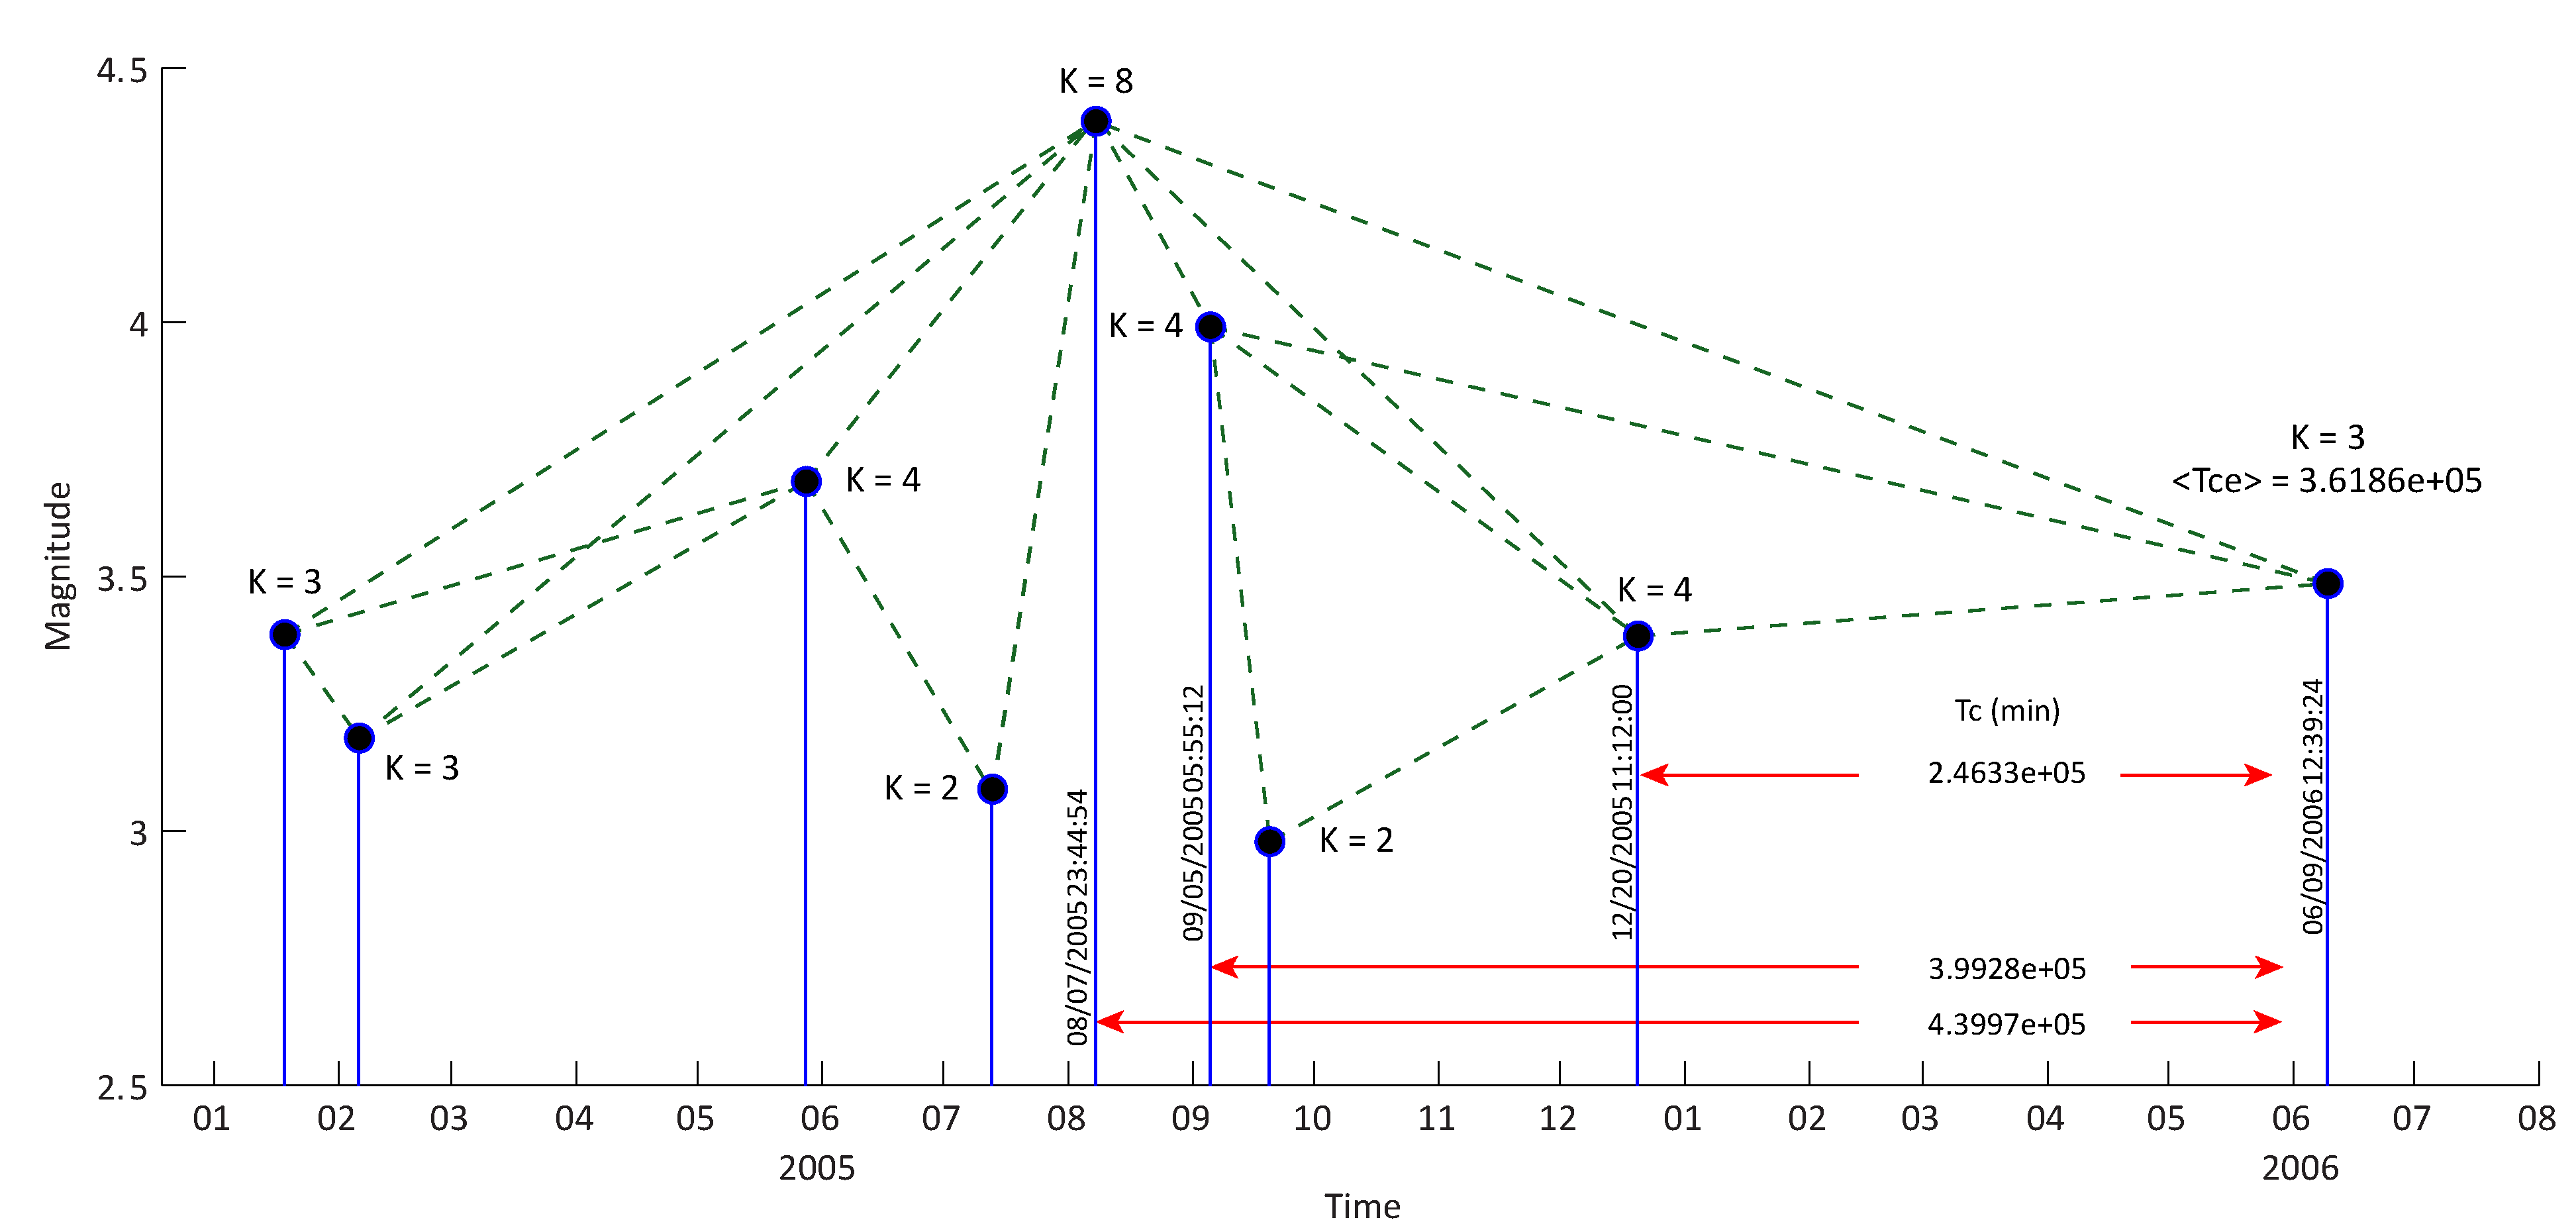
\includegraphics[width=0.8\textwidth]{figures/pdf/Figure01} 
	\caption{Sketch of the VG method. The initial events of Kopeh Dagh region are represented. Couple of events were deleted due to illustration purposes. The blue vertical lines indicate the events. Height of each line is corresponding the magnitude of the event. The green dashed lines show the allowable connections between events. The connectivity degree (K) of each event is presented. The red arrows show the time difference between events. The $T_c$ and $< T_c >$ values of the last event are represented. Note that the mean of all $<T_c>$ values in each window will be the window mean interval connectivity time.}
	\label{fig:vg}
\end{figure*}

Plotting $k$ against magnitude results on a scattered set of points which have been shown to be acceptably represented by a linear correlation, here referred to as the $k$-$M$ relationship, the slope of which also shows a linear relationship with the seismicity $b$-value of the seismic zone under consideration, or a universal sample of $k$-$M$ slope and $b$ values \citep{Telesca2013, Telesca2014}. \citet{Telesca2014} also observed that it was reasonable to draw a relationship between the distribution of the events when considering whether these were connected (visible to each other) or not and time. Let $T_c$ be the interval connectivity time, which is nothing but the time difference between two inter-visible events (see Fig.~\ref{fig:vg}); and <$T_c^e$> be the average of all $T_c$ values computed for event $e$; then it is possible to compute the visibility graph mean interval connectivity time <$T_c$>, which is the mean value of all <$T_c^e$> in a given time sequence of events.

Because <$T_c$> can be obtained for any sub-graph within a larger graph, that is, for any time window in a larger magnitude-time series of events, then it is possible to investigate the evolution of <$T_c$> (and that of the $k$-$M$ slope and the $b$-value) for a moving window sliding along the magnitude-time series. When doing so, \citet{Telesca2014} suggested to associate the values of each sub-sequence with the last event in the sequence. Following this approach, \citet{Telesca2014, Telesca2016} found that the variation of <$T_c$> over time exhibited a possible relationship with the occurrence of earthquakes. This and the aforementioned relationship between the $k$-$M$ slope and the $b$-value are aspects we explore next for our region and earthquake-sequence of interest.

% Fig.~\ref{fig:vg} shows initial events of KopehDagh magnitude-time series with connectivity degree of each event. 




\section{Tectonic seismic regions and seismicity parameters}

The Iranian plateau is located on the Himalayan-Alpine seismic belt. It has a long history of large magnitude ($M>7$) earthquakes that are well documented dating back to the eighth century. Based on seismicity parameters and the geologic provinces of the plateau, Iranian earthquakes have been categorized into various seismic zones, ranging from the definition of four to nine major seismic zones in the more traditional studies \citep[e.g.,][]{Stocklin1968,Takin1972,Berberian1976}, and up to twenty to twenty-three tectonic seismic regions in the most elaborate ones \citep[e.g.,][]{Nowroozi1976,Tavakoli1999}. \citet{Mirzaei1998},  dividing Iran into five tectonic regions, called Azerbaijan-Alborz, Kopeh-Dagh, Zagros, Central-East Iran, and Makran. Considering the division of  \citet{Mirzaei1998} as a reference,  \citet{Karimiparidari2013}  divided the Azerbaijan-Alborz tectonic seismic region into two regions, which are Azerbaijan and the Alborz Mountain Range (hereinafter, Alborz). Azerbaijan, Alborz, and Kopeh-Dagh tectonic seismic regions encompass most of northern Iran.  Fig.~\ref{fig:study_region} shows the study area and tectonic seismic regions.
 
\begin{figure*}[t]
	\centering
	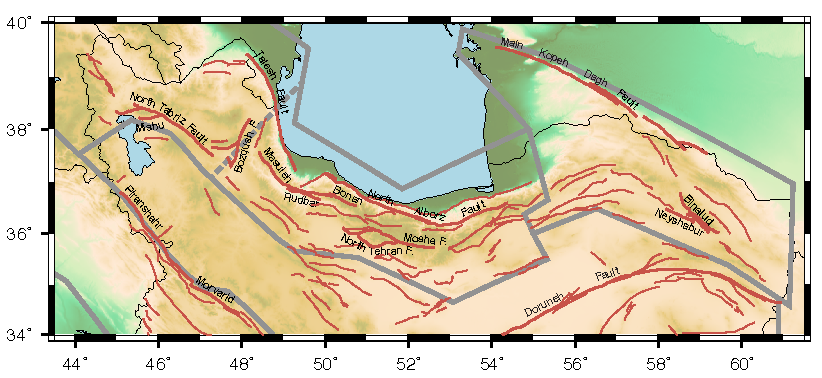
\includegraphics[width=0.75\textwidth]{figures/pdf/Figure02} 
	\caption{Region of interest and tectonic seismic regions. At the top, the map of Iran and surrounding countries is presented. The study area is located in the gray box. At the bottom, the study area containing seismotectonic provinces after \citet{Mirzaei1998} is presented. Dashed line is the subdivision that is proposed by \citet{Karimiparidari2013}}
	\label{fig:study_region}
\end{figure*}
  
The Alborz tectonic seismic region has active reverse faults, which are parallel to the northwest-trending structural gain of the Alborz Mountains belt. The North Tehran Thrust adds more complexity due to the presence of south-dipping reverse faults, which are in part blind, such as the Davudieh, Shian, and Bagh-E Feyz. The northwest continuation of the Alborz Mountains, known as the Rocks of the Talesh Mountains, have been thrust northeastward and eastward over rocks of the south Caspian depression  \citep{Berberian1999}.\\ 
The Tabriz region (located in the Azerbaijan tectonic seismic region) is in the Araxes structural block of northwestern Iran, southwest of the continuation of the western Alborz Mountains toward the Caucasus. The North Tabriz Fault (NTF) is a complex northwest-trending structure, which contains evidence observed on aerial photographs, and vertical displacement with the north side up, of right-lateral strike-slip displacement  \citep{Berberian1999}.

The main Kopeh-Dagh fault consists of several partly overlapping segments parallel to the overall  NW - SE  structure with step-overs. The regions of overlap are characterized by shorter south-dipping thrust faults, striking roughly E - W  \citep{Berberian2001}.  \citet{Trifonov1978} reported active displacement along the main Kopeh-Dagh fault for more than 500 km. Main fault lines and fault systems in the interest region is represented in Fig.~\ref{fig:faults}.

\begin{figure*}[t]
\centering
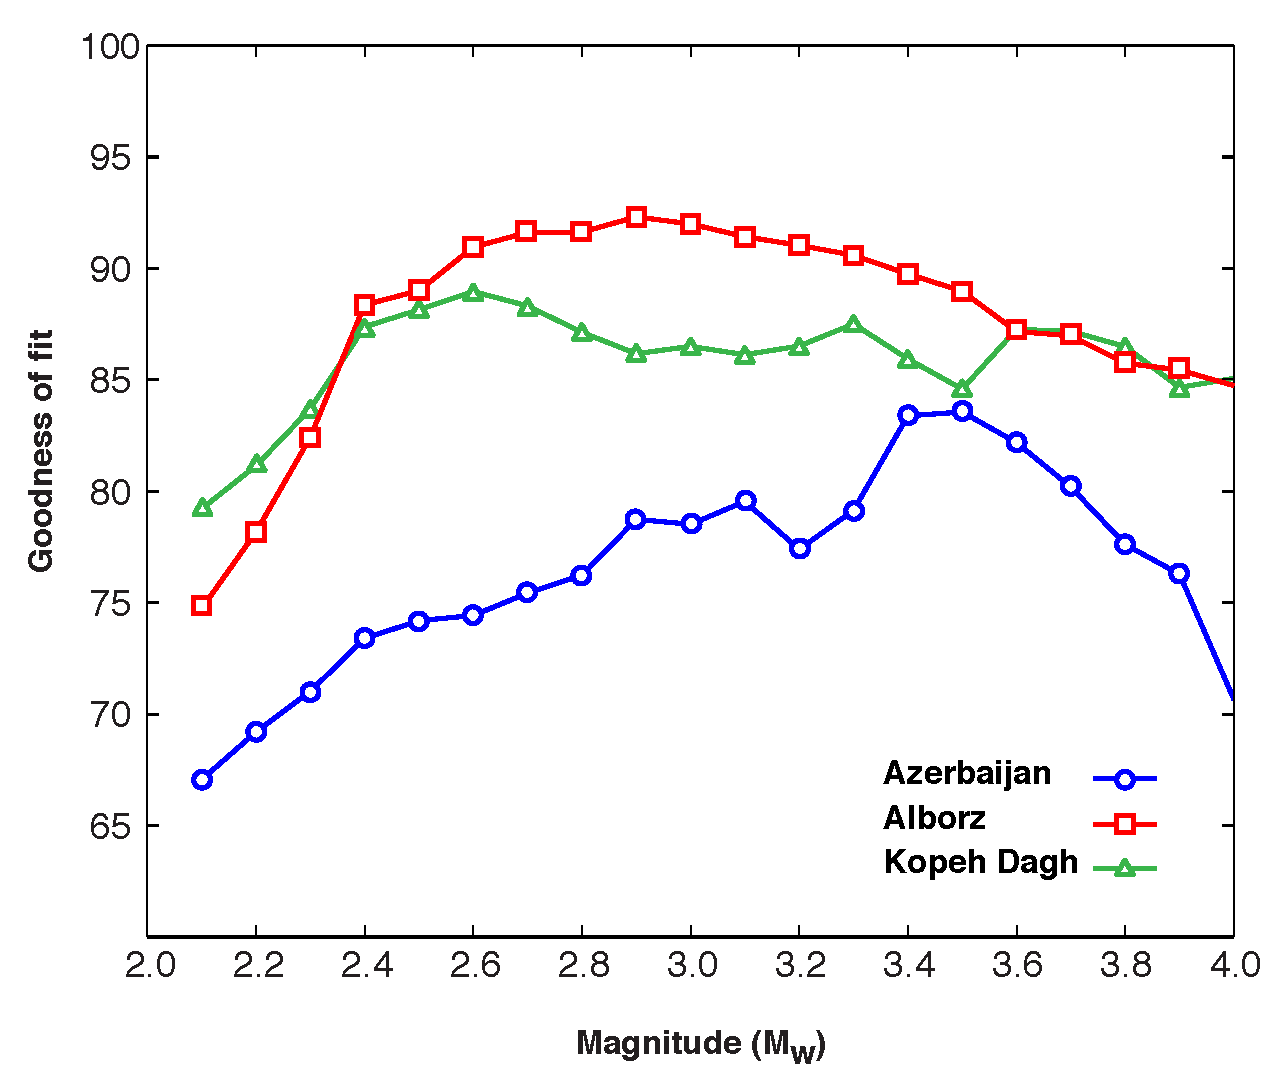
\includegraphics[scale=1]{figures/pdf/Figure03.pdf} 
\caption{Main fault line and fault system in the region of interest. The borderlines of the seismic zones shown in Fig.~\ref{fig:study_region} are shown in background in gray.}
\label{fig:faults}
\end{figure*}

\subsection{Magnitude Conversion}

The catalog of recorded earthquakes from 2005-15, downloaded from IIEES, reported earthquakes based on different magnitude scales \citep{IIEES}. The  $M_L$,  $M_S$, and  $mb$  magnitudes were converted through conversion relationships, as defined in  \citet{Zare2014}. Some data were also recorded in  $M_D$  (duration magnitude). These data are reported by the International Seismological Centre (ISC).   \citet{Deniz2010}  developed a set of empirical equations to convert earthquake magnitudes from  $mb$,  $M_D$,  $M_L$, and  $M_S$  scales to  $M_W$  scale using the orthogonal regression procedure. They used data from different data centers, including the ISC, of earthquakes that occurred in Turkey. In this study, we use the conversion equation of  \citet{Deniz2010}  to convert  $M_D$  to  $M_W$. 

\subsection{Declustering} 

It is generally assumed that the seismicity of each tectonic seismic source follows a Poissonian occurrence process. Therefore, in order to accomplish this, we decluster the earthquake catalog. In compiling the catalog of events, foreshocks and aftershocks are removed using a declustering methodology  presented by \citet{Gardner1974}. Fig.~\ref{fig:seismicity}  shows the epicenter of declustered instrumental  earthquakes.

\begin{figure*}[t]
\centering
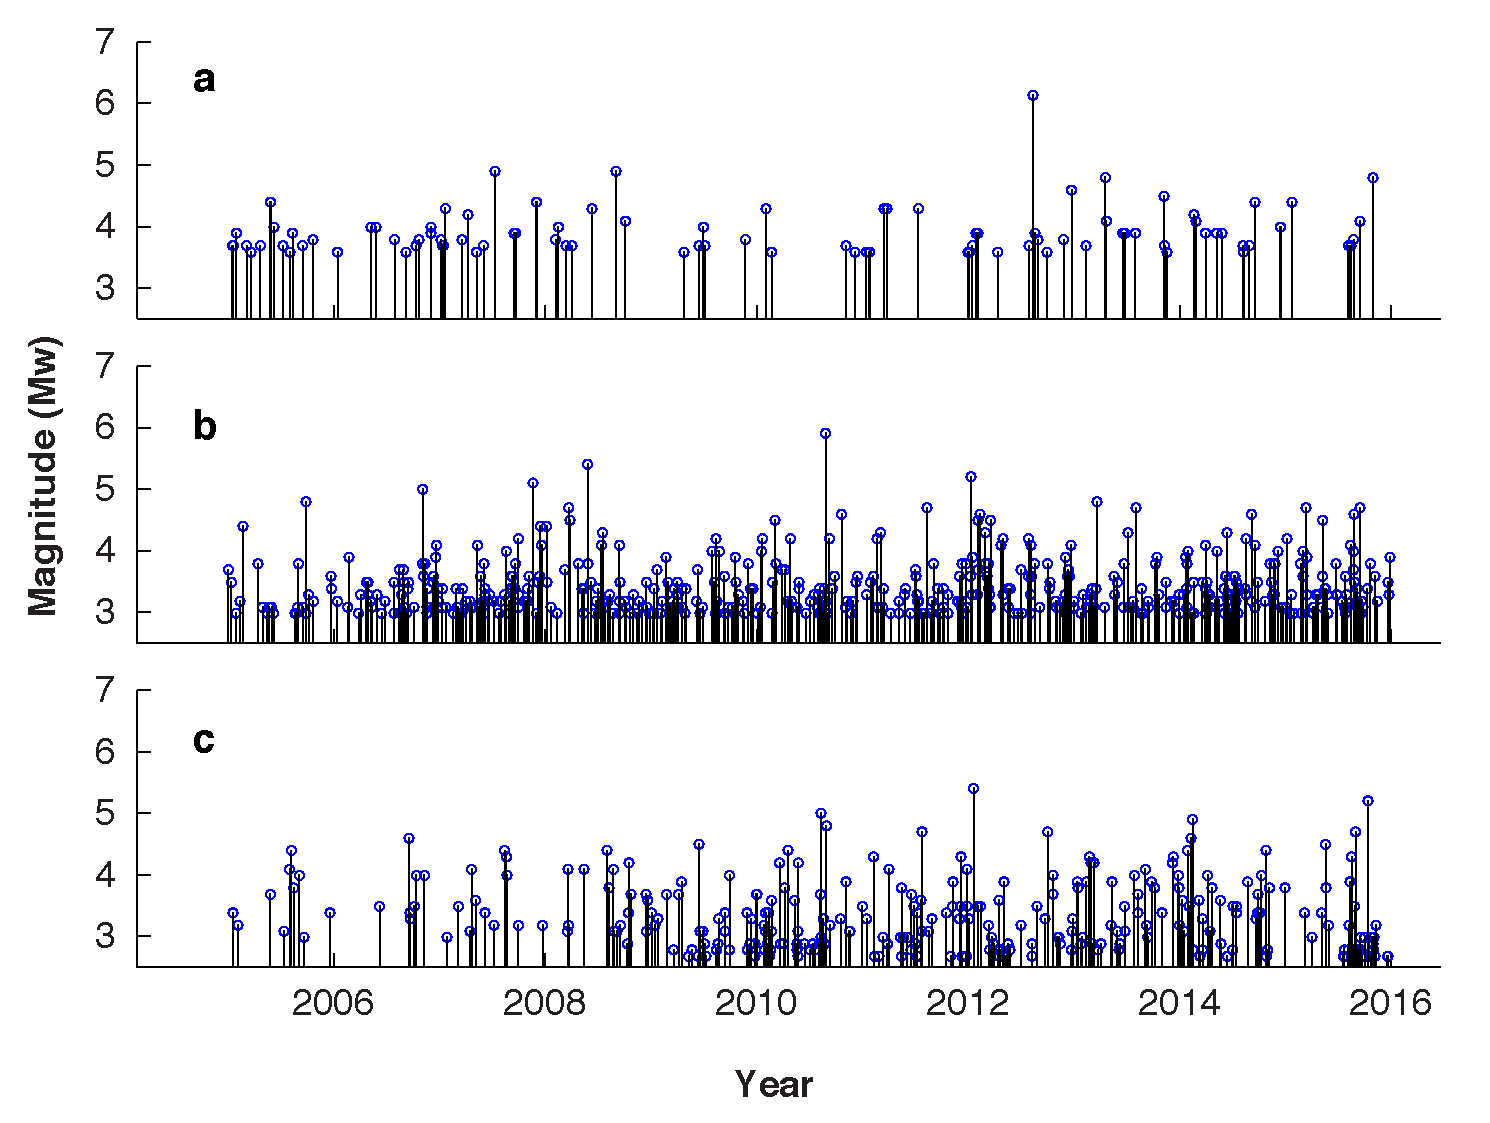
\includegraphics[scale=1]{figures/pdf/Figure04.pdf} 
\caption{Declustered instrumental seismicity map (2005 - 2015) of northern Iran. Different colors indicate the seismicity of different regions. Size of symbols are proportional to the magnitude of the events.}
\label{fig:seismicity}
\end{figure*}
 
\subsection{Catalog Completeness}

Catalog completeness is an important factor in studying an earthquake sequence. This characteristic measured as the minimum magnitude of complete recording for earthquake catalog. The completeness magnitude $(M_c)$ is often determined using simple numerical analysis. Two common approaches are maximum curvature method (MAXC) and goodness-of-fit test (GFT)(see \citet{Wiemer2000}). We use the Goodness-of-fit test and compute $M_c$ for each region's catalog. According to the GFT method, a complete catalog should follow the Gutenberg-Richter power law distribution of magnitude. The steps for selecting the completeness magnitude for each catalog include: 1) calculating the a-  and  b-  value based on minimum magnitude; 2) generating  synthetic events based on the achieved value when the cumulative number of events obey the power law distribution; and 3) calculating goodness of fit for predicted and observed cumulative numbers for each magnitude bin  \citep{Wiemer2000}. We increase the minimum magnitude and repeat the process in order to calculate the goodness of fit for each magnitude.  \citet{Wiemer2000} assumed a goodness of fit of 90\% as a threshold to select the completeness of the catalog. However,  not all frequency-magnitude distributions reach the 90\% mark. Fig.~\ref{fig:completeness} shows the goodness-of-fit values for three tectonic seismic regions. For each tectonic seismic region, we select the magnitude corresponding to the highest goodness of fit or the first magnitude with the goodness of fit greater than 90\%.

\begin{figure}[t]
\centering
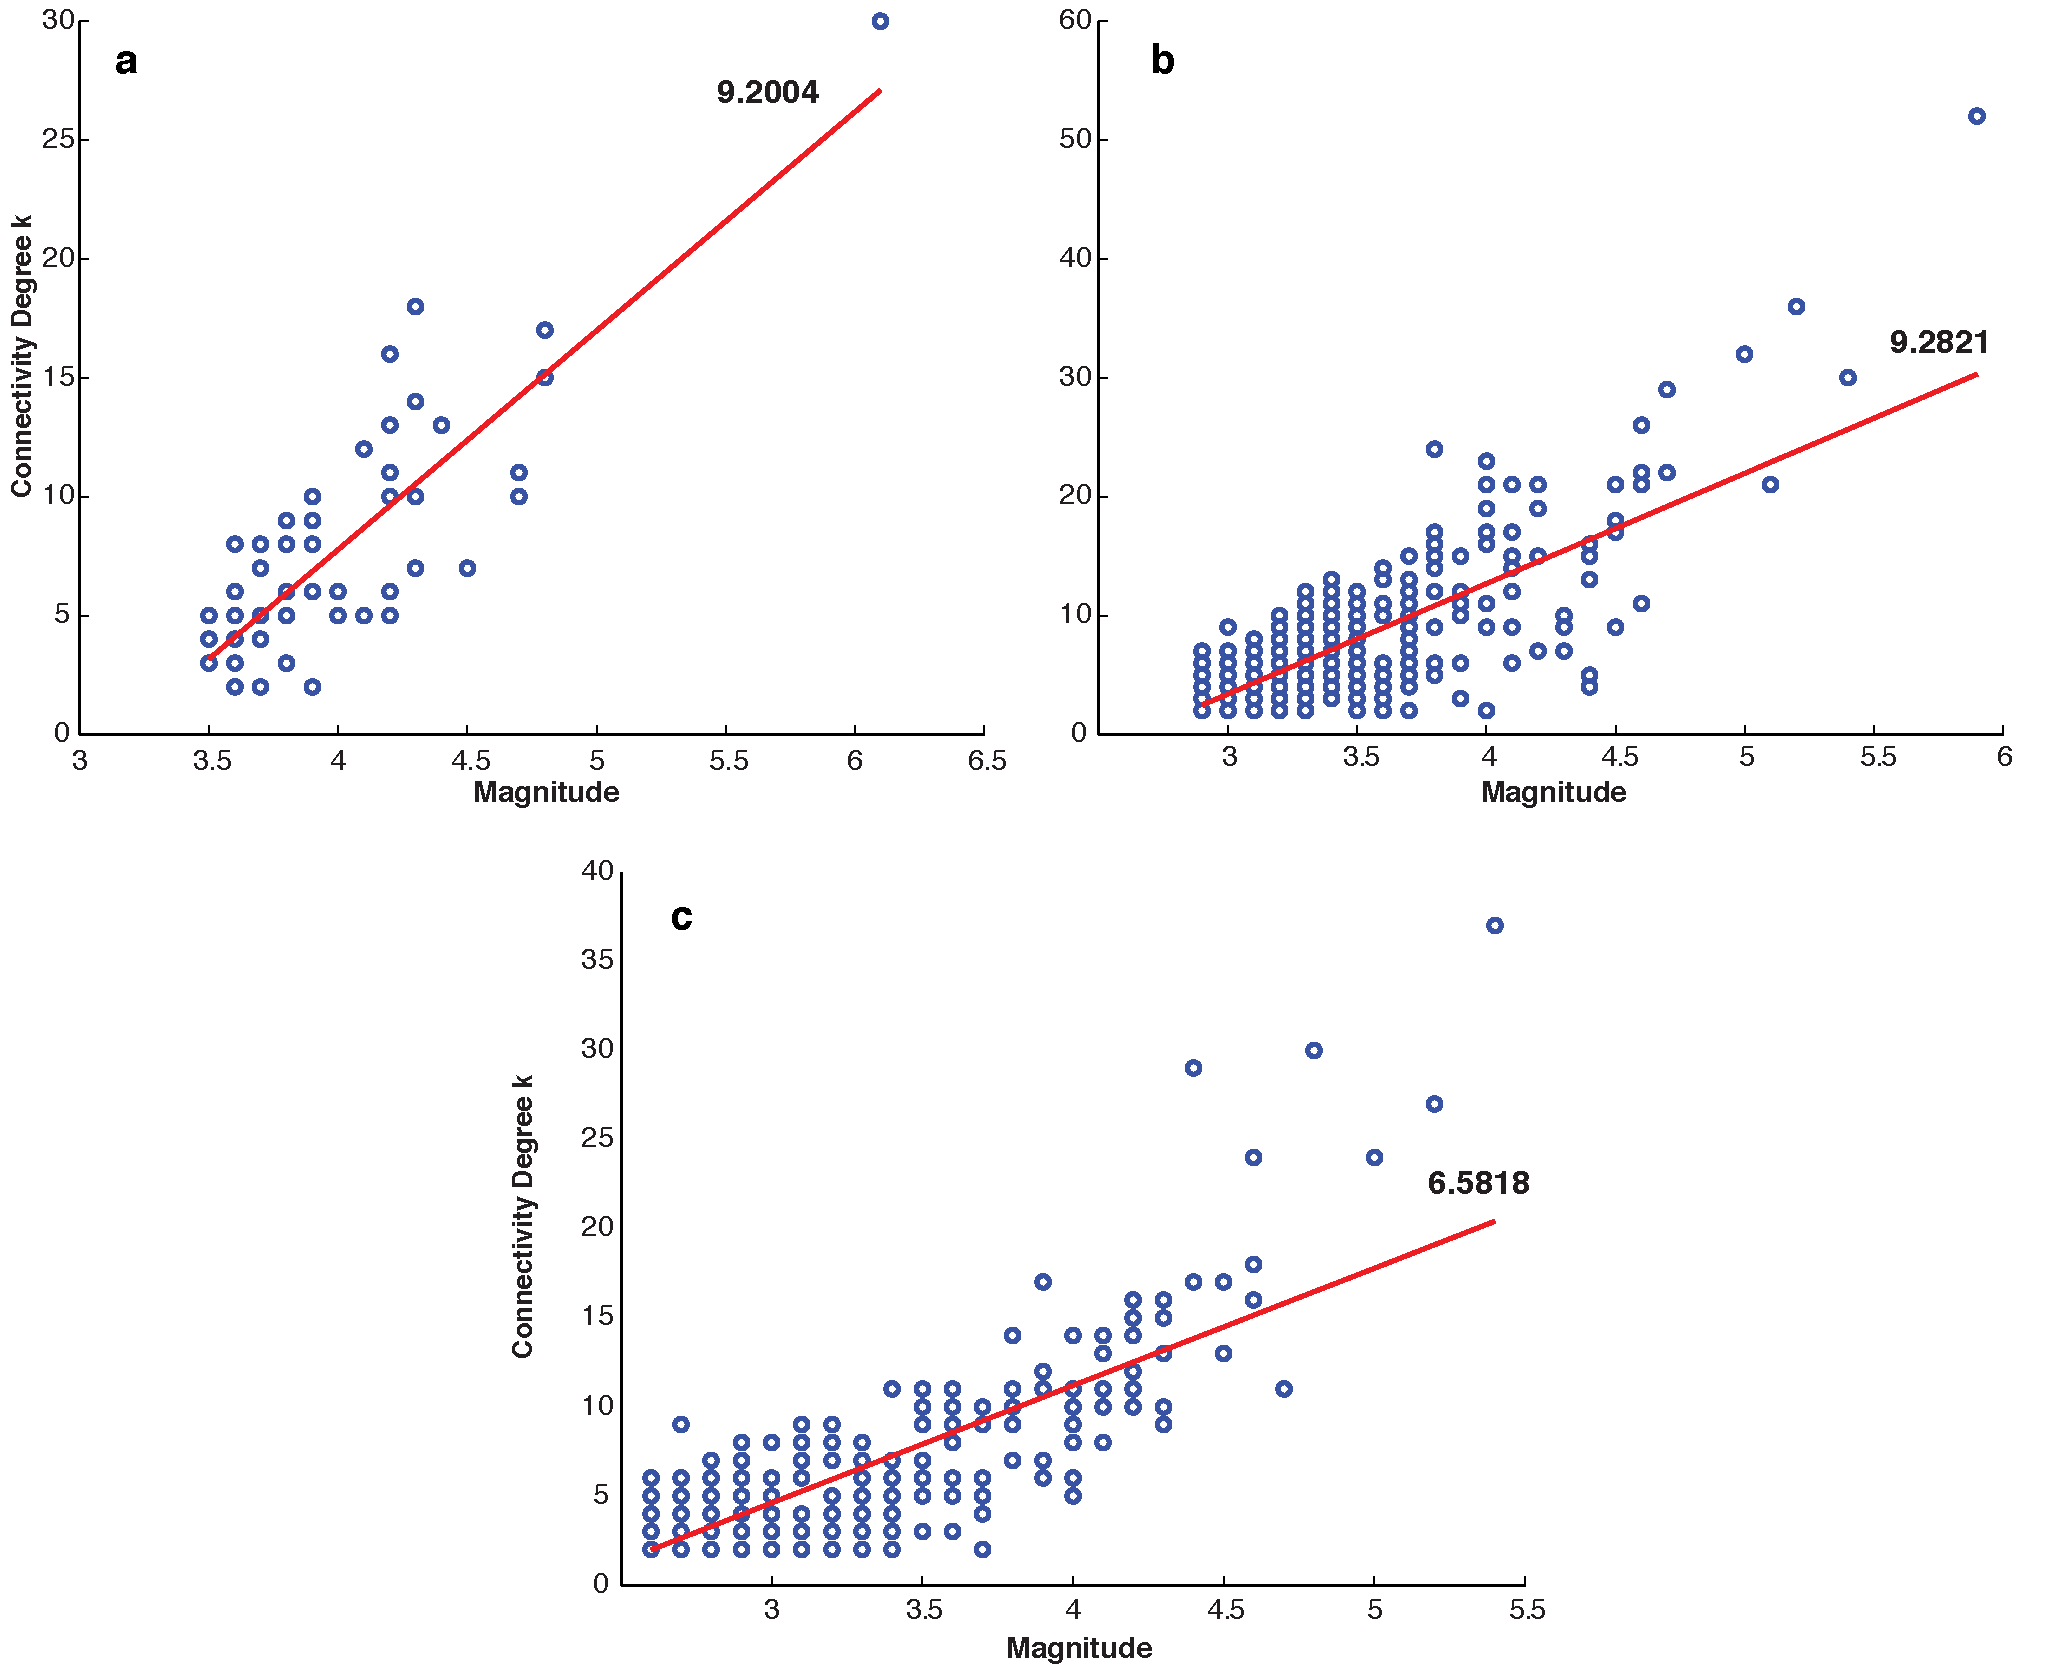
\includegraphics[width=0.45\textwidth]{figures/pdf/Figure05.pdf} 
\caption{ Selection of completeness magnitude $M_c$ of the three tectonic seismic regions in northern Iran in 2005-15 period. The symbols indicate the computed GFT values as function of the earthquake magnitude. The horizontal dashed line indicates the desired threshold for the goodness of fit value at 90 percent. The vertical dashed lines indicate the completeness magnitude of each tectonic seismic region.}
\label{fig:completeness}
\end{figure} 

Based on the results represented in Fig.~\ref{fig:completeness}, we select the minimum magnitudes for complete recording,  $M_c$ , is 3.5, 2.6, and 2.6 for Azerbaijan, Alborz, and Kopeh Dagh, respectively. Fig.~\ref{fig:mag-time}  shows the magnitude time series of the declustered data for the three regions. Earthquakes with magnitude greater than the completeness magnitude are represented. 

\begin{figure*}[t]
	\centering
	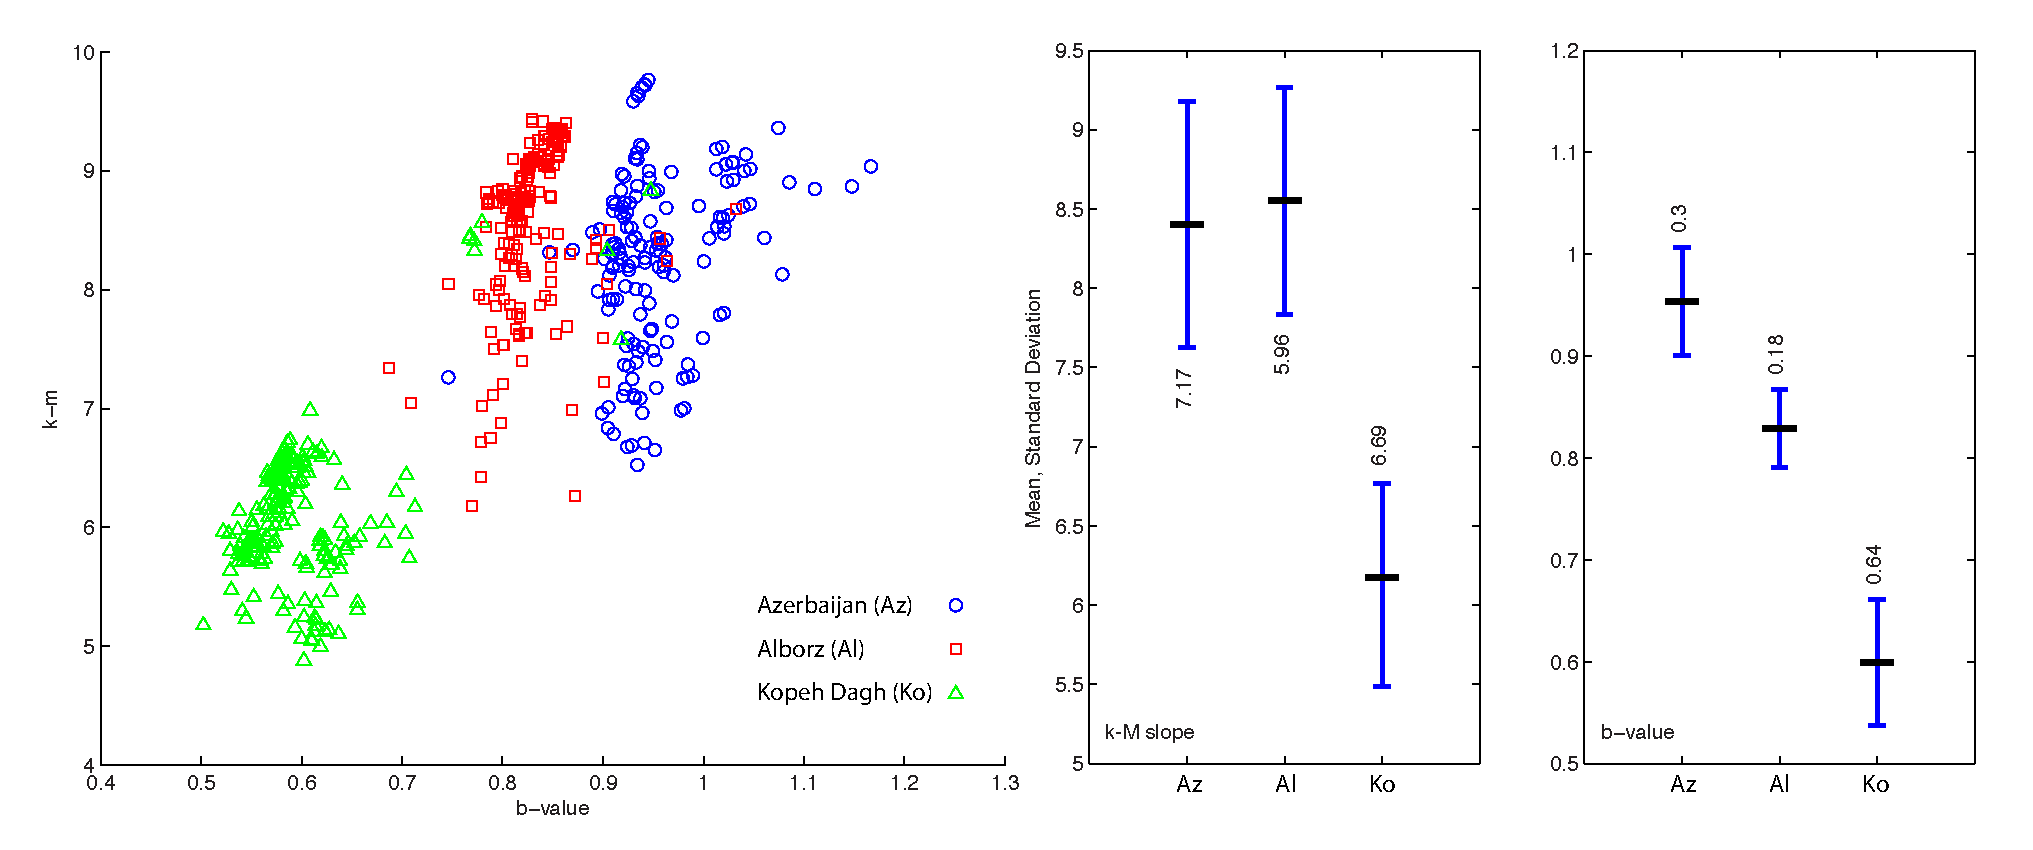
\includegraphics[scale=0.8]{figures/pdf/Figure06.pdf} 
	\caption{Variation of moment magnitude ($M_w$) of 2005-2015 earthquake for north Iran as a function of time. The figure only represents the declustered events greater than minimum magnitude. The 2012 $M_w 6.4$ East Azerbaijan, 2010 $M_w 5.8$ Damghan, and 2012 $M_w 5.4$ Neyshabur earthquakes are clearly visible as maximum values in Azerbaijan (Az),  Alborz (Az), and Kopeh Dagh (Ko) magnitude-time series.}
	\label{fig:mag-time}
\end{figure*}



% 
\section{Results}

We generate the visibility graphs for each sub-region of interest using the time-magnitude sequences \myrevision{of both the complete and declustered catalogs. In the case of the complete catalog, that corresponds to the sequences shown in Fig.~\ref{fig:mag-time}. In every case, the numbers of nodes in each graph are the same as those shown in Table \ref{tab:seismicity}; and} the links between inter-visible events are established following the condition in equation (\ref{eq:vg}), as in the example shown in Fig.~\ref{fig:vg}. (We do not include a visualization of the graphs because the links are so many, that it is only practical to visualize the graphs of short sequences.) We collect information about the number of inter-visibility links associated with each event (connectivity degree, $k$) and categorize the events in magnitude bins of size $\Delta M_{\mathrm{bin}} = 0.1$, as mentioned in the Methodology section. Figure \ref{fig:km} shows the scattered distribution of events in the magnitude-connectivity degree plane for each sub-region\myrevision{, corresponding to the complete catalogs.} The figure shows that, in general, the value of $k$ increases with $M_w$\myrevision{; and includes the results of obtaining linear $k$-$M$ regressions for each dataset along with the values of the $k$-$M$ slopes for the three seismic zones, namely 10.0, 9.85, and 8.70 for the Azerbaijan, Alborz, and Kopeh Dagh regions. Similar results regressions were obtained for the declustered catalogs, which yielded slopes of 8.92, 8.97, and 7.96, respectively.}

\begin{figure*}[t]
	\centering
	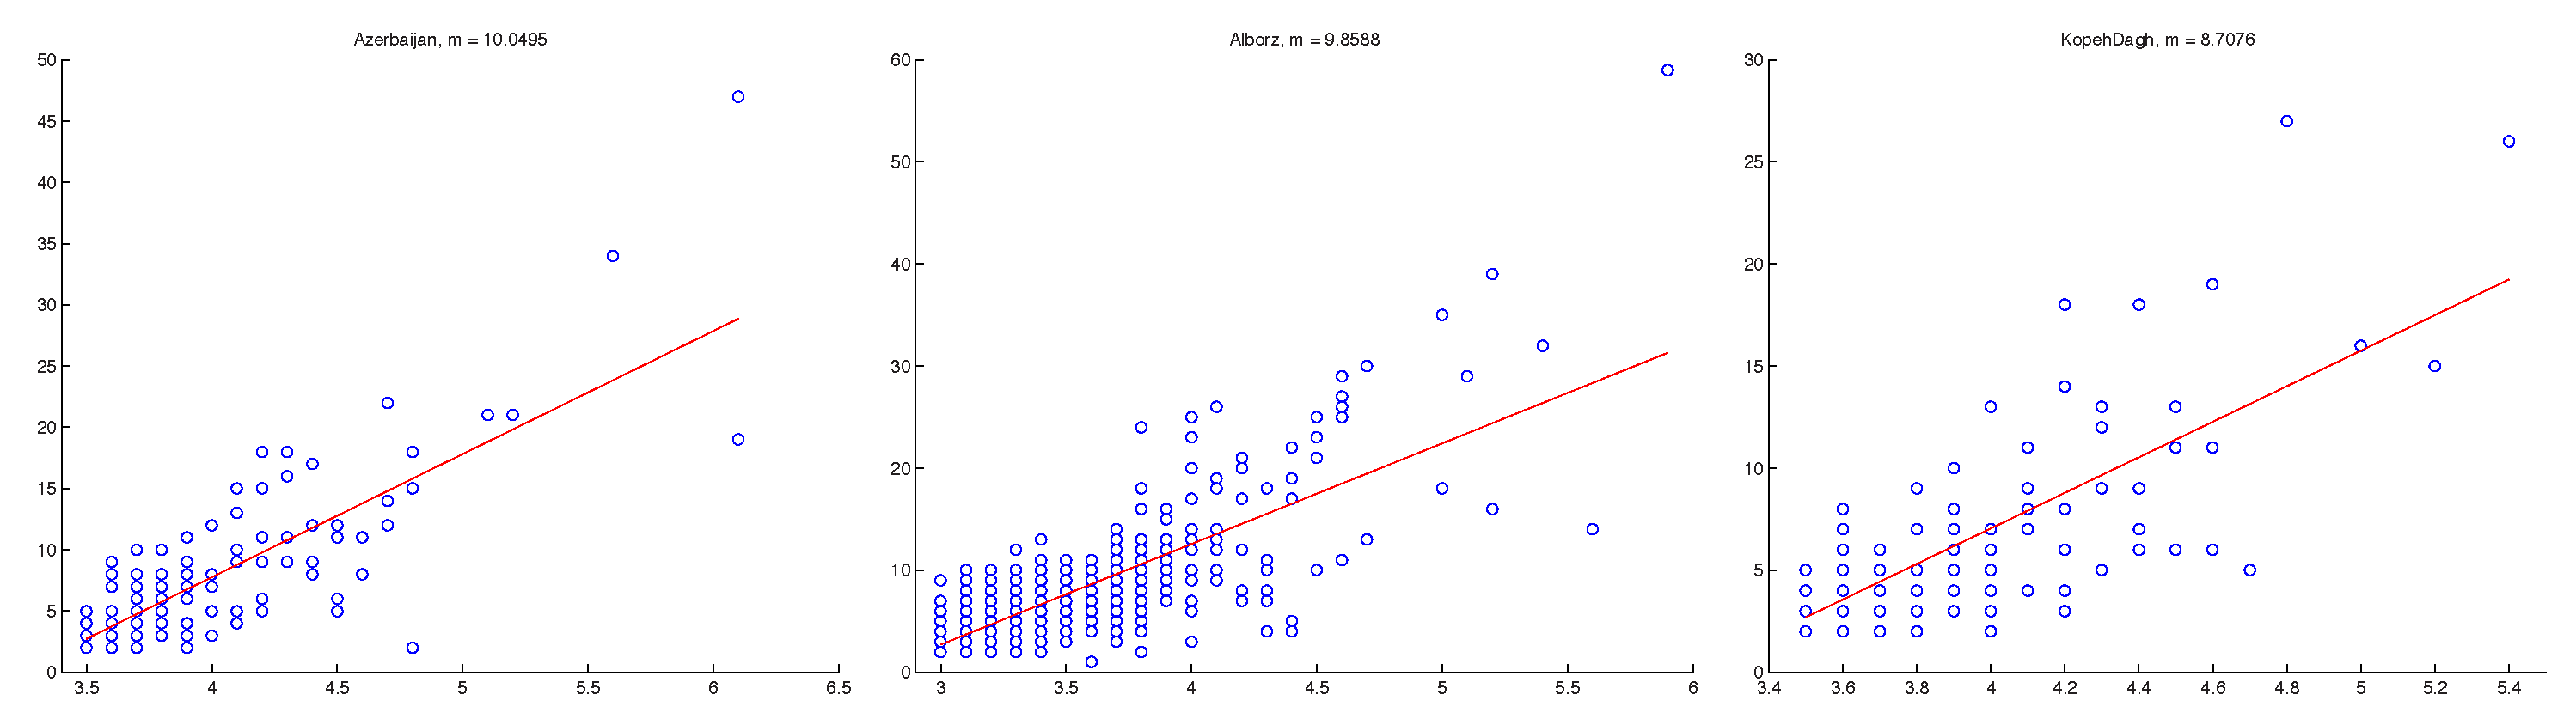
\includegraphics[width=\textwidth]{figures/pdf/figure-06-rev.pdf} 
	\caption{Scattered distribution of events in the magnitude-connectivity degree plane and linear regressions obtained for the $k$-$M$ relationships for the three seismic regions in northern Iran. The value next to each of regression line corresponds to the slope of the line, which is referred here as the $k$-$M$ slope. The color version of this figure is available only in the electronic edition.}
	\label{fig:km}
\end{figure*}

Next, we examine the relationship between the $b$-values from Table \ref{tab:seismicity} and the $k$-$M$ slopes. 

* * *

\myrevision{The $b$-value, by definition, represents the proportion between the amount of large events and that of small events.} Fig.~\ref{fig:regression} shows the scattered results for $k$-$M$ slope versus $b$-value for the three tectonic seismic regions in northern Iran along with the data-points obtained for the analysis of the magnitude-time sequences of the Mexican subduction zone \citep{Telesca2013} and the Pannoninan seismic zone \citep{Telesca2014}, as well as other experimental results \citep{Telesca2014-pone}. \myrevision{According to Scholtz (1968) b-value for microfractures in rocks is reported ranging between 0.11 and 2.58. Using different synthetic and real catalog, in this study we cover a broad range from low b-value (synthetics) to high b-value(subduction zone)}. Fig.~\ref{fig:regression} also includes the results of different linear regressions between the $b$-value and the $k$-$M$ slope. Each regression reflects the addition of new data-points from different studies. Note that the regression improves as new data-points are added, which is indicated by the correlation coefficient $R$, also included in the figure. The correlation fitting various regional seismic data was previously pointed out by \citet{Telesca2014}.

According to these results, a universal relationship between the $b$-value and the $k$-$M$ slope ($m$) can be expressed as:
% 
\begin{equation}
	b = 0.073 + 0.084 m \, .
	\label{eq:universal.bm}
\end{equation}

\begin{figure}[h]%[t]
	\centering
	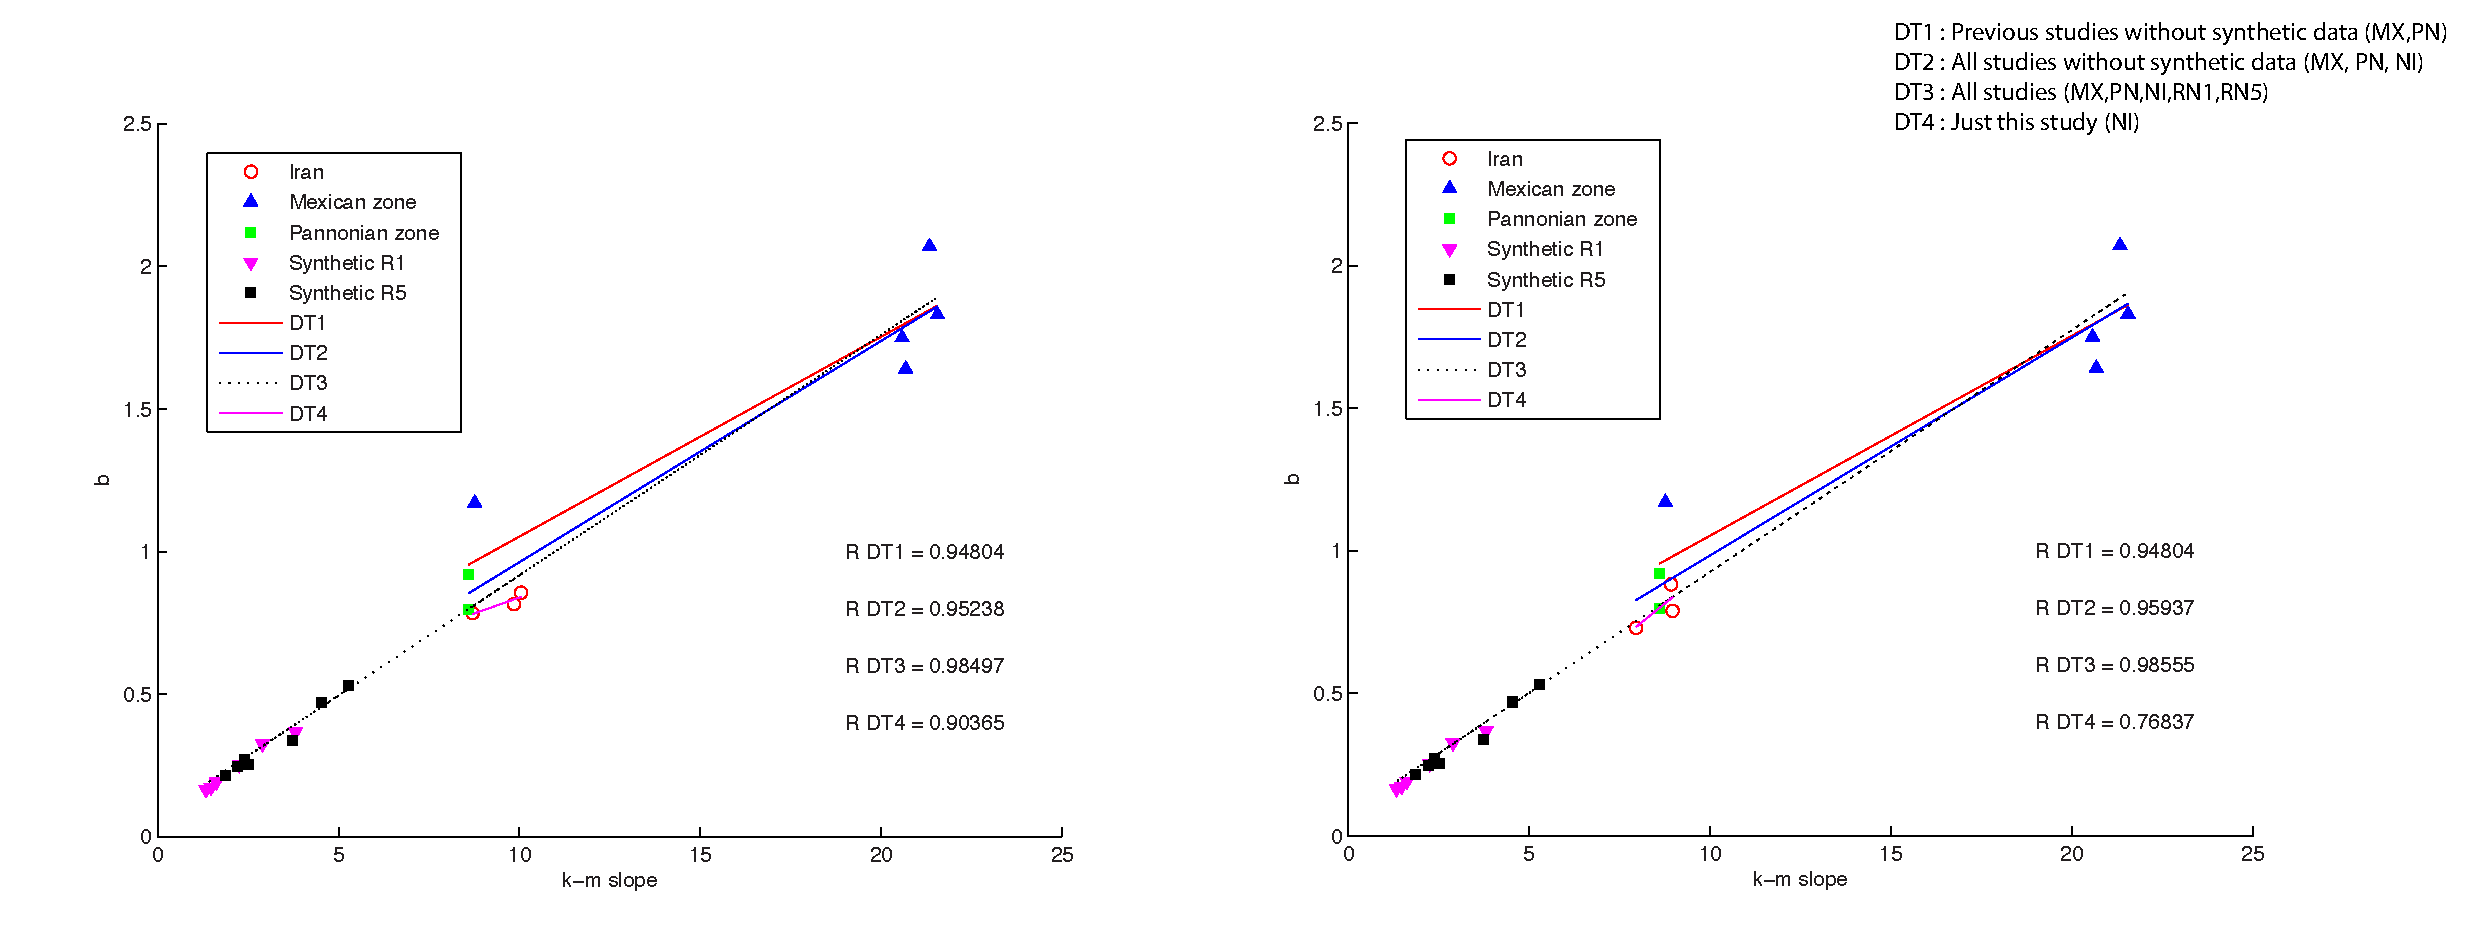
\includegraphics[width=0.45\textwidth]{figures/pdf/figure-07-rev.pdf} 
	\caption{Correlation between $k$-$M$ slope and $b$-value as drawn from the results of the present study for the region of northern Iranian and three other previous studies, including analysis of the Mexican subduction zone \citep{Telesca2013}, the Pannonian seismic zone \citep{Telesca2014}, and results from two experiments \citep{Telesca2014-pone}. The lines represent linear regressions obtained to fit the different data points, considering different combinations. The values of the correlation coefficient, $R$, are indicated for each regression line. The color version of this figure is available only in the electronic edition.}
	\label{fig:regression}
\end{figure}

Another aspect of interest is the stability of the data points themselves. Note that as presented in Fig.~\ref{fig:regression}, the analysis of the sequences shown in Fig.~\ref{fig:mag-time} only contribute one data point per region of interest. Furthermore, each data-point comes from sequences that vary significantly in terms of the number of events and seismic parameters (see Table \ref{tab:seismicity}). 

\citet{Telesca2013} observed that the value of the $k$-$M$ slope is not particularly sensitive to the sample size in the sequence---at least not when considering sufficiently large sequences. On the other hand, as we will see below, if the sequence window is sufficiently small, then the $k$-$M$ slope value shows a relative dependence on time and thus provides insight about the variation of the seismicity as the sequence progresses. 
% \cmmnt{Note also that the threshold value of $M_c$ is significantly smaller for Azerbaijan than for Alborz or Kopeh Dagh. This is due in part to the fact that the latter two zones were more seismically active in the time period under consideration} 
\myrevision{In this study due to using windowing method, we consider a very conservative completeness magnitude}. However, according to \citet{Telesca2012}, the threshold magnitude has a minor effect in the graph parameters.

To further explore the sensitivity of the graph properties to the number of events in each catalog and the value of the minimum magnitude, we randomly picked a significant number of sub-sequences from within the initial catalog compiled for each region, and repeated the analysis for each sub-sequence. In total, for each region, we extracted 200 new sub-sequences from the \myrevision{whole} catalog. The number of events in each sub-sequence was varied randomly but chosen to be large enough to represent the seismic characteristics of each region. In particular, the minimum size of each sub-sequence was set to be $n \geq 200$, and the maximum size in the sequence was set to be as large as the original catalog (\myrevision{whole catalog}; see Table \ref{tab:seismicity}). We forced the random sub-sequences to progress positively in time without altering the natural occurrence of events. In other words, we randomly determined the initial event and the sub-sequence size (number of events to be considered), and then picked that number of events following the initial earthquake in the sub-sequence. Next, we determined the value of $M_c$ and $b$ as previously done for the complete catalogs, created the graph for all events with $M \geq M_c$, and extracted the connectivity degree of the events in each sub-sequence. \myrevision{Note that the results of the whole catalog for each seismic region is different from Fig.~\ref{fig:regression}. In Fig.~\ref{fig:regression} we choose a time dependent completeness magnitude which is conservative and requires inspection. In order to keep uniformity in the random data test we computed the completeness magnitude through GFT for all subsamples and the whole catalog of each seismic region. Determination of completeness magnitude based on the best score of GFT between synthetic catalog and subsamples could be controversial. It is possible to choose very large $M_c$ just because of slightly higher GFT score than smaller magnitudes. This could result in a sequence  of data where is not completely a representative of the domain. However, knowing these source of uncertainties, the randomly generated data conforms the fact that the method is fairly robust for the catalog size and completeness magnitude; where we can easily distinguish the 3 seismic region border. There are some outlier data due to subsamples of aftershocks of big earthquakes. These sequences represent different $k-M$ and $b-value$ relationship. These sequences do not represent the dominant seismicity pattern of the region. In the declustered catalog (is not presented here) we do not see these outliers.}

\begin{figure*}%[t]
	\centering
	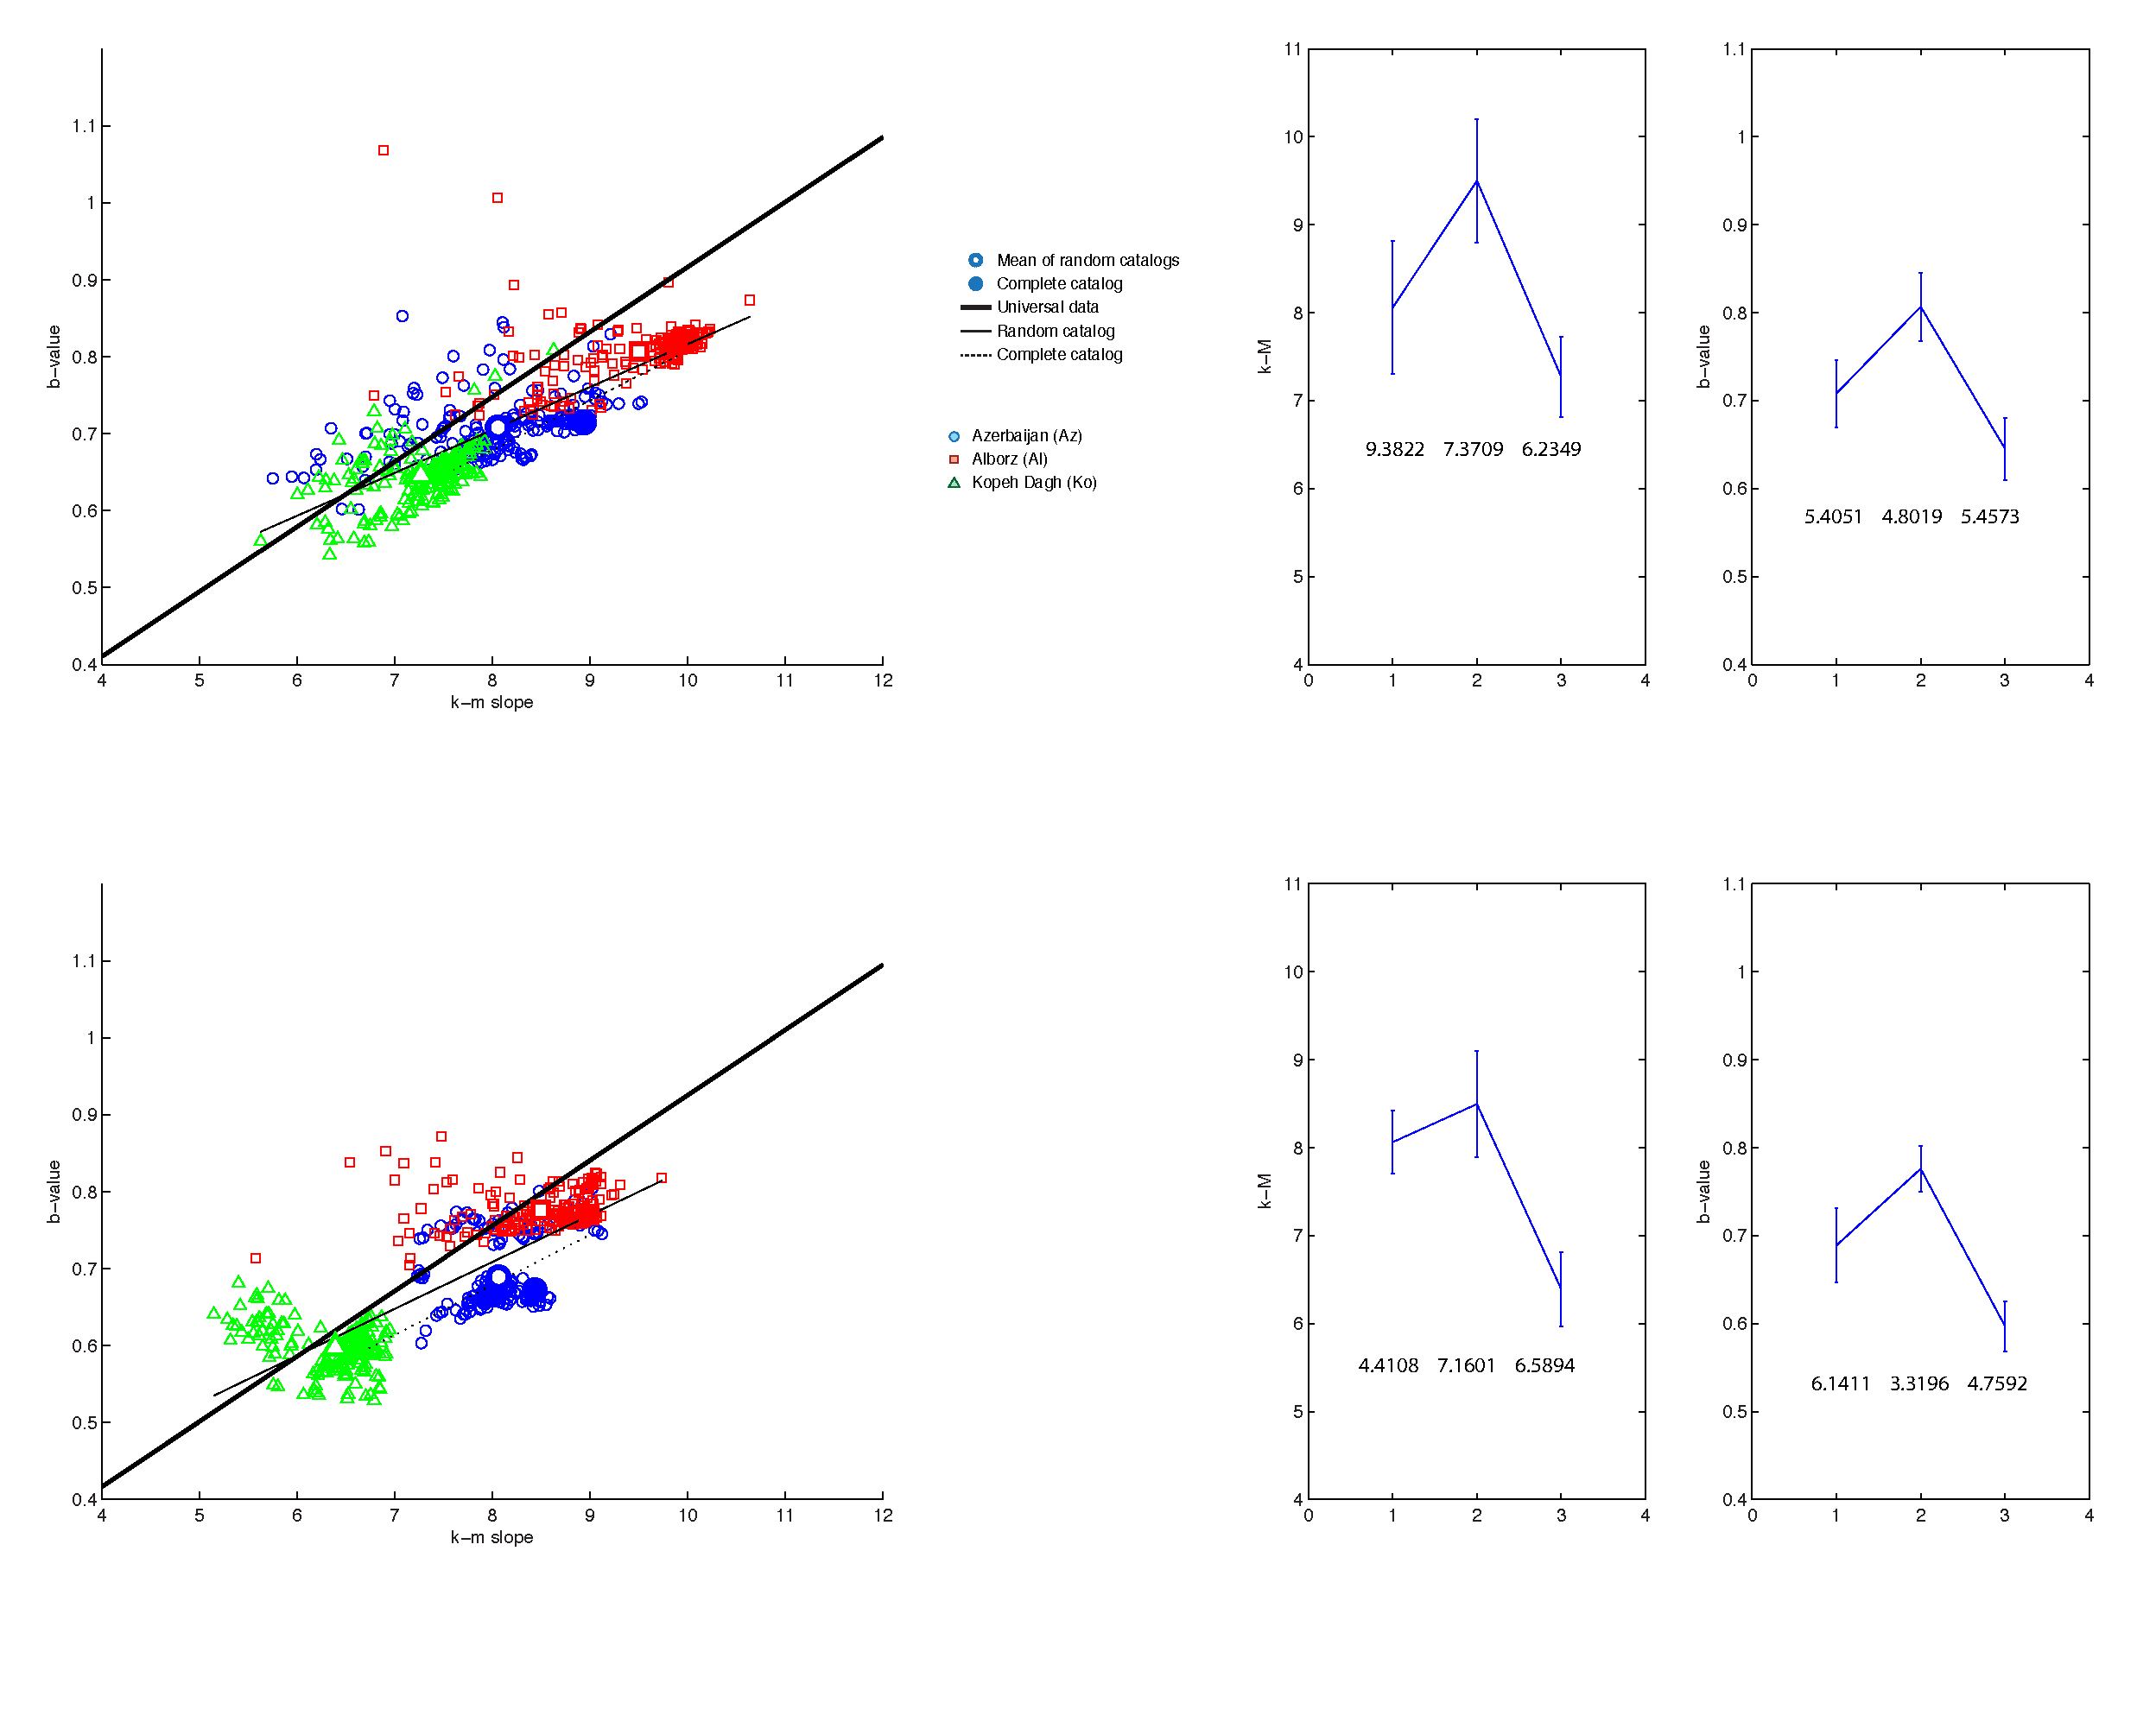
\includegraphics[width=0.9\textwidth]{figures/pdf/figure-08-rev.pdf} 
	\caption{\textbf{(a)} Correlation between $k$-$M$ slope and $b$-values for 200 random sequences extracted from the \myrevision{whole} catalogs of the three northern Iranian seismic regions considered in this study (scattered symbols), including the mean values (empty symbols with thick border) and the data points obtained from the analysis of the complete catalog (solid symbols), along with the linear regressions of each sample as indicated in the legend. \textbf{(b)} Mean, $\pm1$ standard deviation, and coefficient of variation (in percent) for the $k$-$M$ slope values of the three seismic zones in northern Iran. \textbf{(c)} Same as part (b), but corresponding to the $b$-value. The color version of this figure is available only in the electronic edition.}
	\label{fig:random}
\end{figure*}

Fig.~\ref{fig:random}a shows scattered points for all the individual $k$-$M$ slope and $b$-value pairs for all the sub-sequences that were randomly picked from the initial catalogs of each region in northern Iran (small symbols). Figures \ref{fig:random}b and \ref{fig:random}c show the variability of the $k$-$M$ slope and $b$-value, respectively. These latter figures show the mean values of each parameter for all the random sub-sequences and the amplitudes of $\pm 1$ standard deviation, as well as the coefficients of variation (in percentage). Figure \ref{fig:random}a also includes the data points corresponding to the complete catalogs (large solid symbols); the points corresponding to the mean values of the $k$-$M$ slope and $b$, from Figs.~\ref{fig:random}b and \ref{fig:random}c (large hollow symbols); and the universal linear regression from equation (\ref{eq:universal.bm}) (thick line), as well as the linear regressions for northern Iran when using the complete catalogs (dashed thin line) and the random sub-catalogs (continuous thin line). 

The comparison between the mean values of the random sequences analysis versus the complete catalogs presented in Fig.~\ref{fig:random} indicates that there exists only a small bias, which is well within the standard deviation of the different value samples. We note that the values of the $k$-$M$ slope are slightly smaller when obtained with the random sequence analysis, whereas the $b$ values seem more stable. 

% \cmmnt{
% The comparisons of the regressions, however, indicate that the analysis of the random sub-catalogs leads to a result more in line with the universal results obtained when considering multiple seismic zones. The linear regression of the random sub-catalogs yields the following equation:
% % 
% \begin{equation}
%    	b = 0.045  +0.390 m \, .
% 	\label{eq:iran.bm}
% \end{equation}

% Note that equations (\ref{eq:universal.bm}) and (\ref{eq:iran.bm}) have similar intercepts with the $b$-value axis, and only slightly different slope constants. In this particular case, the analysis for northern Iran leads to a relationship in which the $b$-value increases more rapidly with $m$ than in the case of the regression obtained for the universal data. The similarity between the two equations, however, is a positive sign of the stability of the method.}

\begin{figure*}%[t]
	\centering
	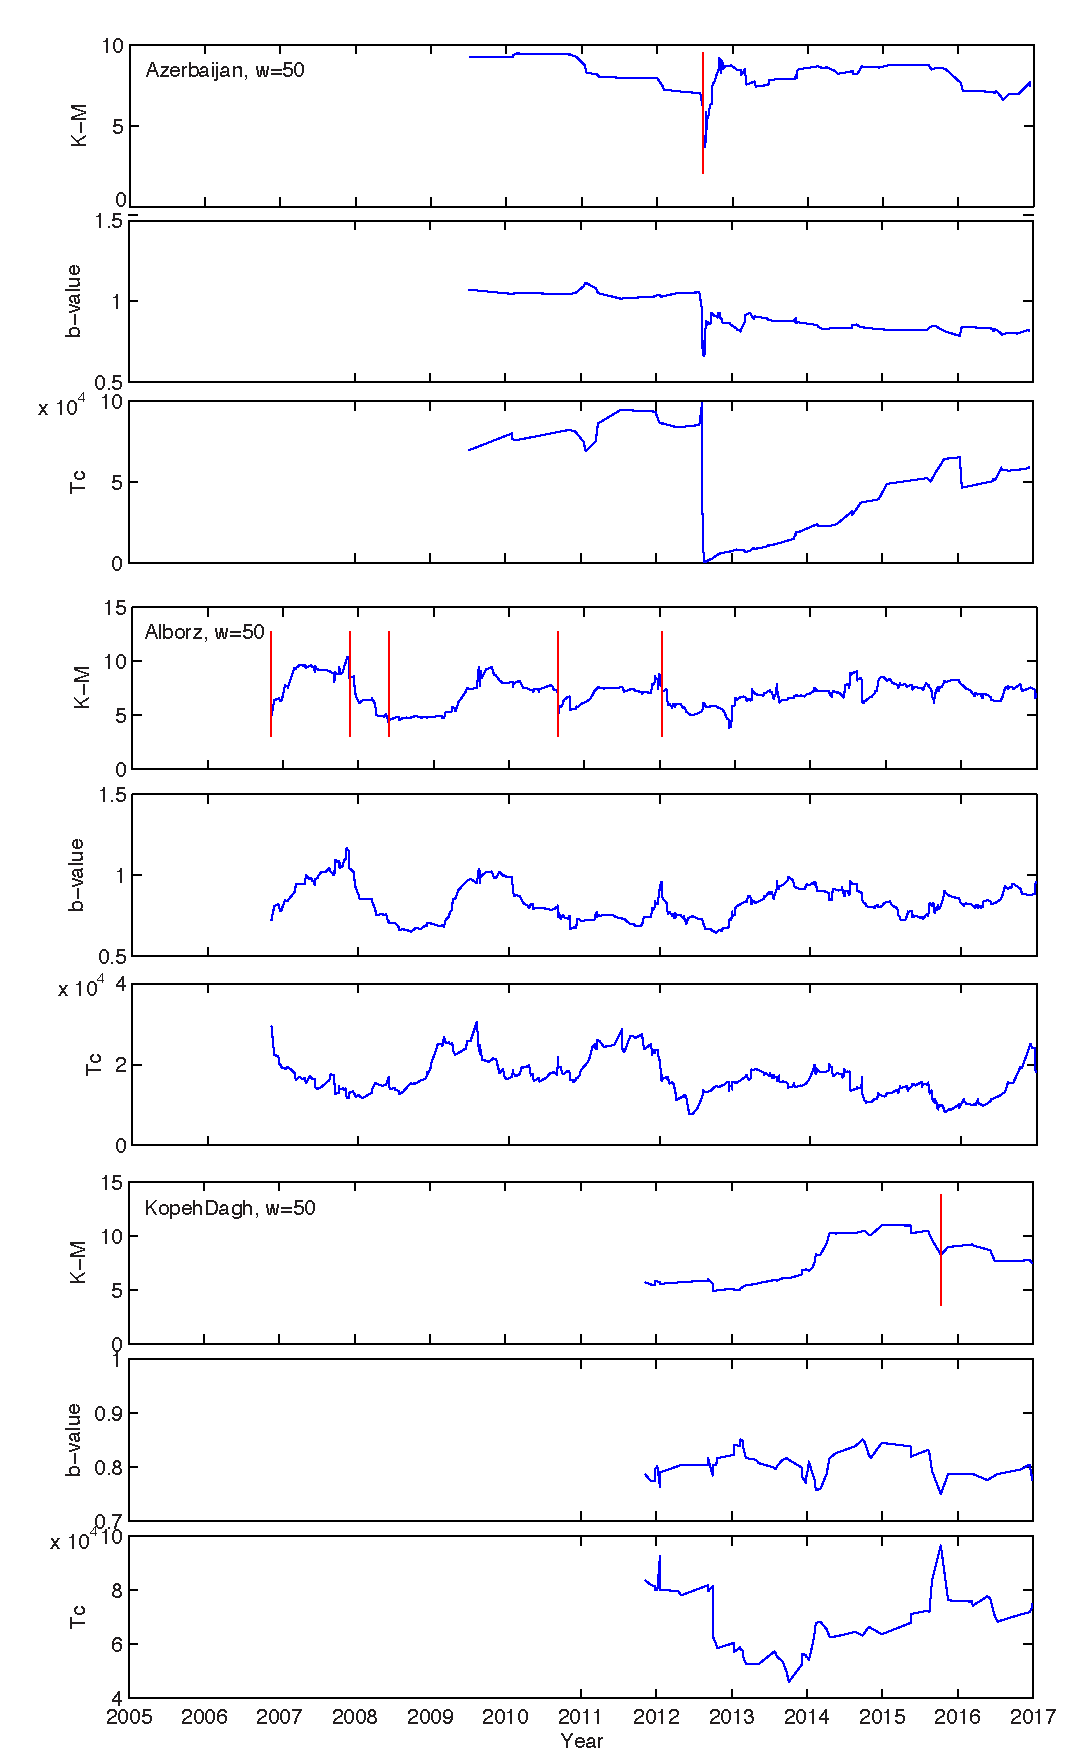
\includegraphics[width=0.75\textwidth]{figures/pdf/figure-09-rev.pdf} 
	\caption{Variation of <$T_c$>, $k$-$M$ slope and $b$-value as with respect to time for three seismic zones for a moving window analysis of the visibility graphs of sub-sequences of \myrevision{50} consecutive events, along with the magnitude of events in the 2005--\myrevision{2016} period. Black triangles indicate the occurrence of major earthquakes in each of the regions, with the corresponding magnitude at the top of each symbol. In the middle frame of each region, the dashed line corresponds to the $k$-$M$ values, whereas the continuous plot shows the variation of the $b$-value. The color version of this figure is available only in the electronic edition.}
	\label{fig:tc}
\end{figure*}

We now investigate the relationship of the parameters obtained through the visibility graph analysis with time. Here, the visibility graph analysis is done by windows of equal number of events moving in time across the catalog sequence. The number of events in the window is kept fixed independently of the time between them, and the results are associated with the last event in the window. In this case, we are interested in using a small number of events to capture the relevance of each new event as the window moves in time. We tried different \myrevision{window size (20-100 events per window) for each seismic zone. The characteristics of major events are not considerably changing due to window size. There is a trade of in choosing the window size. Small windowing size will highlight the local changes in the time series, however, in the mean time it won't represent a true seismicity characteristic of the subsample (e.g., b-value). We choose window size as 50 to be small enough to represent the variation of k-M, b-value and Tc in time and large enough in agreement with Woessner and Wiemer (2005) who found that at least the number of events has to be 50 to get reliable estimate of b-value.} At this point it is also of interest to compute the value of <$T_c$> explained in the Methodology section.

Figure \ref{fig:tc} shows the variation of <$T_c$>, the $k$-$M$ slope, and the $b$-value with time for each of the three seismic zones in northern Iran. The time-magnitude sequence is also included for reference. Note that the behavior of the $k$-$M$ slope and the $b$-value is very similar along time for all three zones. \myrevision{Specially in the case of Alborz where because of higher number of events the correlation is easily seen.} This is consistent with the results presented before. We note that there seems to be a correlation between the behavior of the $b$-value in time with the occurrence of some of these larger events. In particular, some of the events in the figure seem to coincide with a drop in the $b$-value. 

The decline of the $b$-value before large earthquakes has been studied in other regions before \citep[e.g.,][]{Wyss2000, Wyss2006, Schorlemmer2005, Chan2012}. In the context of the visibility graph analysis, \citet{Telesca2016} observed a decrease in <$T_c$> before the large earthquake of the western India earthquake sequence. We recognize, however, that the lack of larger ($M>6$) events in our region of interest in the last decade prevents us from drawing a stronger conclusion on this regard. 


% 
\section{Conclusions}

We studied the seismicity of the three main seismic regions in northern Iran in the time period between January 2005 and December \myrevision{2016} using an approach based on the visibility graph method. We tested the applicability of this method for the specific region of interest and in reference to previous results from similar studies. The results confirm previous observations about the correlation that exists between the connectivity parameter $k$, the magnitude of the events in the sequence, \myrevision{the slope $m$ of the linear regression adjusted to the relationship between $k$ and $M$, and the correlation of the $b$-value from the Gutenberg-Richter law with $m$. We used the data points computed from the visibility graph analysis of the seismicity of northern Iran to obtain updated mathematical expressions for a universal relationship between $b$ and $m$, including data collected from previous studies done} for other regions as well as data from experiments. We found the relationships to have a good level of similarity, \myrevision{independently of the alternative manipulations of the seismic catalog, but noted that the results were somewhat sensitive to the completeness magnitude. Overall, our results are} indicative of the general nature of the relationship between $m$ and $b$. We also explored the relationships \myrevision{between the visibility graph properties and the seismicity parameters for a random selection of earthquake subsequences and for a progression of subsequences in time. In these cases, we found the relationship between $b$ and $m$ to hold for subsequences with a sufficiently large number of events ($n \geq 50$), but noticed they are in better agreement with the universal regressions when larger, entire regional sequences are considered. Unfortunately, for the particular regions considered in this study, we were not able to detect conclusive evidence of other relationships between the visibility graph properties and the temporal occurrence of large earthquakes, as it has been suggested in previous similar studies. We believe this is due to the lack of larger magnitude events ($M_w > 6$) in the selected catalogs.}

\myrevision{While the connection between the topological properties of the visibility graph of an earthquake sequence and the seismicity parameters of a region is an attractive finding, it remains to be seen how this can be put to use in a more practical scientific sense. We believe future efforts in understanding the mathematical nature of the observed relationships is a natural first step to follow. It will also be necessary to test the relationships in additional seismic regions with uncharacteristic $b$ values, especially in the ranges outside the typical $b$-values (0.8--1.2). It would also be of interest to build visibility graphs based on other earthquake parameters (e.g., moment) or considering directionality, and investigate other relationships. At this point, nonetheless, the method as used here} seems to provide an alternative and interesting approach to the analysis of the seismicity of a region.

% OLD MATERIAL
% -----------------------------------------------------------------

% that can be drawn from a moving window visibility graph analysis and the variation of the seismicity in the region of interest in time. \myrevision{We found that the }

% \myrevision{The relationship found between k-M slope and b-value suggest that the topological properties of the VG are not unlinked with the seismological properties of  an earthquake sequence.} 

% We found there may be a potential relationship between the $b$ value and the occurrence of earthquakes as well as with the graph's mean interval connectivity time parameter <$T_c$>, but additional research in regions with stronger events may be necessary before drawing stronger conclusions in this regard. \myrevision{Also further investigation has to be performed in the future to clarify the relationship between the k-M slopes as a pure mathematical object and the b-value and investigate the k-M slope with other earthquake network models.} The method used here, nonetheless, seems to provide an alternative and interesting approach to the analysis of the seismicity of a region. 

% We studied the earthquake sequence of three tectonic seismic regions of northern Iran. Results manifest the strong relationship between  $k-M$  slope and Gutenberg-Richter parameters. The variations of  $k-M$  slope and  b-value  with time in sliding windows have similar behavior and decline before large earthquakes. A significant reduction of  $<T_c>$  value before large earthquakes was observed. The higher coefficient of variation of  $k-M$  slope in comparison with  b-value  suggests that the  $k-M$  slope is a better parameter for studying the magnitude time series due to higher sensitivity to window size and threshold magnitude than  is found in the $b-value$. Sensitivity analysis revealed that the VG parameters behave independently than threshold magnitude and number of events. In general,  the $k-M$  and  $b-value$  relationship preserves the behavior with the variation in the window size and threshold magnitude, and could be an alternative approach for clustering earthquake sequences based on different tectonic seismic zones.


\section{Data and Resources}

Data used to compile the seismic catalog employed in the analysis was obtained using the Web browser search application from the International Institute of Earthquake Engineering and Seismology, IIEES (\url{http://www.iiees.ac.ir/en/eqcatalog/}, last accessed September 2016). The raw versions of figures were prepared using MATLAB\textsuperscript{\textregistered}, release 13b; and the Generic Mapping Tools, version 5.1 \citep[\url{http://gmt.soest.hawaii.edu;}][]{Wessel_2013_EOS}. Final versions of figures were prepared using Adobe\textsuperscript{\textregistered} Illustrator\textsuperscript{\textregistered}.

% \manuscriptadjust
% 
\section{Acknowledgments}

This research was possible thanks to support from the Center for Earthquake Research and Information (CERI) at the University of Memphis. CERI is designated as a Center of Excellence by the Tennessee Board of Regents and is funded in part by the State of Tennessee under State Sunset Laws (SB 1510 and HB 1608, 2015--2016).


\manuscriptadjust
\setlength{\bibsep}{0pt}
\bibliographystyle{mybssabib}
{\small\bibliography{references}}


% \section{Introduction}
% \label{sec:introduction}
% Your text comes here. Separate text sections with
% \section{Section title}
% \label{sec:1}
% Text with citations \cite{RefB} and \cite{RefJ}.
% \subsection{Subsection title}
% \label{sec:2}
% as required. Don't forget to give each section
% and subsection a unique label (see Sect.~\ref{sec:1}).
% \paragraph{Paragraph headings} Use paragraph headings as needed.
% \begin{equation}
% a^2+b^2=c^2
% \end{equation}

% % For one-column wide figures use
% \begin{figure}
% % Use the relevant command to insert your figure file.
% % For example, with the graphicx package use
%   \includegraphics{example.eps}
% % figure caption is below the figure
% \caption{Please write your figure caption here}
% \label{fig:1}       % Give a unique label
% \end{figure}
% %
% % For two-column wide figures use
% \begin{figure*}
% % Use the relevant command to insert your figure file.
% % For example, with the graphicx package use
%   \includegraphics[width=0.75\textwidth]{example.eps}
% % figure caption is below the figure
% \caption{Please write your figure caption here}
% \label{fig:2}       % Give a unique label
% \end{figure*}
% %
% % For tables use
% \begin{table}
% % table caption is above the table
% \caption{Please write your table caption here}
% \label{tab:1}       % Give a unique label
% % For LaTeX tables use
% \begin{tabular}{lll}
% \hline\noalign{\smallskip}
% first & second & third  \\
% \noalign{\smallskip}\hline\noalign{\smallskip}
% number & number & number \\
% number & number & number \\
% \noalign{\smallskip}\hline
% \end{tabular}
% \end{table}


%\begin{acknowledgements}
%If you'd like to thank anyone, place your comments here
%and remove the percent signs.
%\end{acknowledgements}

% BibTeX users please use one of
%\bibliographystyle{spbasic}      % basic style, author-year citations
%\bibliographystyle{spmpsci}      % mathematics and physical sciences
%\bibliographystyle{spphys}       % APS-like style for physics
%\bibliography{}   % name your BibTeX data base

% Non-BibTeX users please use
% \begin{thebibliography}{}
% %
% % and use \bibitem to create references. Consult the Instructions
% % for authors for reference list style.
% %
% \bibitem{RefJ}
% % Format for Journal Reference
% Author, Article title, Journal, Volume, page numbers (year)
% % Format for books
% \bibitem{RefB}
% Author, Book title, page numbers. Publisher, place (year)
% % etc
% \end{thebibliography}

\end{document}

